\documentclass[a4paper,oneside,12pt]{article}
\usepackage{graphics,multicol}
\usepackage[latin1]{inputenc}
\usepackage[a4paper,margin=2cm,lmargin=2cm,headheight=1pt]{geometry}
\usepackage{fancyhdr}
\usepackage{amsmath,amssymb,amsfonts,amsthm, mathrsfs}
\usepackage{mathtools,bbm}
\usepackage{IEEEtrantools}
\usepackage[]{algorithm2e}
\usepackage{tikz,pgfplots,tkz-graph}
\usepackage{ifthen,calc}
\usepackage{listings,hyperref,float}
\usepackage{epsfig,epstopdf,graphicx}
\usepackage{enumerate}

\pgfplotsset{compat=newest}
\usetikzlibrary{positioning,matrix}
\interdisplaylinepenalty=2500

% Page settings
% \setlength{\oddsidemargin}{0 in}
% \setlength{\evensidemargin}{0 in}
% \setlength{\topmargin}{-0.6 in}
% \setlength{\textwidth}{6.5 in}
% \setlength{\textheight}{8.5 in}
% \setlength{\headsep}{0.75 in}
% \setlength{\parindent}{0 in}
% \setlength{\parskip}{0.1 in}

% Markov symbol X -o- Y
\newcommand{\markov}{\mathrel{\multimap}\joinrel\mathrel{-}\joinrel\mathrel{\mkern-6mu}\joinrel\mathrel{-}}
% Independent & not independent symbol X _||_ Y
\newcommand{\indep}{\mathrel{\bot}\joinrel\mathrel{\mkern-5mu}\joinrel\mathrel{\bot}}
\newcommand{\dep}{\centernot\indep}
% i.i.d.
\newcommand{\iid}{\stackrel{\mathrm{i.i.d.}}{\sim}}
% Integration d
\newcommand{\dd}{\mathop{}\!\mathrm{d}}

% Single braces
\newcommand{\agbrs}[1]{\left\langle #1 \right\rangle}	% angle braces,  	< x >
\newcommand{\rdbrs}[1]{\left( #1 \right)}				% round braces,  	( x )
\newcommand{\sqbrs}[1]{\left\lbrack #1 \right\rbrack}	% square braces, 	[ x ]
\newcommand{\clbrs}[1]{\left\lbrace #1 \right\rbrace}	% curly braces, 	{ x }

% Delimited braces
\newcommand{\agbrsv}[2]{\left\lange #1 \,\middle|\, #2 \right\rangle}	% angle braces with delimiter |,  	< x | y >, inner product
\newcommand{\rdbrsv}[2]{\left( #1 \,\middle|\, #2 \right)}				% round braces with delimiter |,  	( x | y ), conditional probability
\newcommand{\sqbrsv}[2]{\left\lbrack #1 \,\middle|\, #2 \right\rbrack}	% square braces with delimiter |,  	[ x | y ], conditional expectation
\newcommand{\clbrsv}[2]{\left\lbrace #1 \,\middle|\, #2 \right\rbrace}	% curly braces with delimiter |,  	{ x | y }, set

% Short for underline and overline
\newcommand{\udl}[1]{\underline{#1}}
\newcommand{\ovl}[1]{\overline{#1}}

% Derivative and partial derivation
\newcommand{\fracd}[2]{ \frac{\mathrm{d} #1}{\mathrm{d} #2} }
\newcommand{\fracp}[2]{ \frac{\partial #1}{\partial #2} }

% Absolute value, norm, ceil, floor, and evaluation
\newcommand{\abs}[1]{\left| #1 \right|}		% Absolute value, 	| x |
\newcommand{\norm}[1]{\left\| #1 \right\|}	% Norm, 			|| x ||
\DeclarePairedDelimiter\ceil{\lceil}{\rceil}
\DeclarePairedDelimiter\floor{\lfloor}{\rfloor}
\newcommand{\eval}[1]{\left. #1 \right|}	% Evaluation, 		f(x) |_{x=x0}

% Definition equal sign
\newcommand{\defeq}{\vcentcolon=}   % :=
\newcommand{\eqdef}{=\vcentcolon}   % =:
\newcommand{\texteq}[1]{\stackrel{#1}{=\joinrel=\joinrel=}}   % use for change of variable

% Inverse hyperbolic functions
\DeclareMathOperator\arcsinh{arcsinh}
\DeclareMathOperator\arccosh{arccosh}
\DeclareMathOperator\arctanh{arctanh}
\DeclareMathOperator\atanh{atanh}
\DeclareMathOperator\sech{sech}

% argmax and argmin
\newcommand\limit[1]{\underset{#1}{\lim}\,}
\newcommand\argmax[1]{\mathrm{arg}\,\underset{#1}{\max}\,}
\newcommand\argmin[1]{\mathrm{arg}\,\underset{#1}{\min}\,}

% Matrices
\newcommand*\pmtx[1]{\begin{pmatrix}#1\end{pmatrix}}			% Matrix with round braces
\newcommand*\bmtx[1]{\begin{bmatrix}#1\end{bmatrix}}			% Matrix with square braces
\newcommand*\vmtx[1]{\begin{vmatrix}#1\end{vmatrix}}			% Determinant of matrix
\newcommand*\spmtx[1]{\rdbrs{\begin{smallmatrix}#1\end{smallmatrix}}}	% Small matrix with round braces
\newcommand*\sbmtx[1]{\sqbrs{\begin{smallmatrix}#1\end{smallmatrix}}}	% Small matrix with square braces
\newcommand*\svmtx[1]{\abs{\begin{smallmatrix}#1\end{smallmatrix}}}		% Determinant of small matrix
\newcommand{\sizecorr}[1]{\makebox[0cm]{\phantom{$\displaystyle #1$}}}	% Get size of an expression

% Theorem environments
\newtheorem{theorem}{Theorem}
\newtheorem{corollary}[theorem]{Corollary}
\newtheorem{lemma}[theorem]{Lemma}
\newtheorem{observation}[theorem]{Observation}
\newtheorem{proposition}[theorem]{Proposition}
\newtheorem{definition}[theorem]{Definition}
\newtheorem{claim}[theorem]{Claim}
\newtheorem{fact}[theorem]{Fact}
\newtheorem{assumption}[theorem]{Assumption}

\newtheorem*{theorem*}{Theorem}
\newtheorem*{corollary*}{Corollary}
\newtheorem*{lemma*}{Lemma}
\newtheorem*{proposition*}{Proposition}
\newtheorem*{definition*}{Definition}
\newtheorem*{example*}{Example}
\newtheorem*{remark*}{Remark}
\newtheorem*{problem*}{Problem}

% Solution environment
\newenvironment{solution}{\begin{proof}[Solution]}{\end{proof}}

% Short for boldsymbol
\newcommand{\bs}[1]{\boldsymbol{#1}}

% Other frequent used operators
\def\Var{\mathsf{Var}}
\def\Cov{\mathsf{Cov}}
\def\coeff{\mathsf{coeff}}
\def\Tr{\mathsf{Tr}}
\def\rank{\mathsf{rank}}
\def\diag{\mathsf{diag}}
\def\mse{\mathsf{mse}}
\def\mmse{\mathsf{mmse}}

\def\ee{\mathbbm{e}}
\def\ii{\mathbbm{i}}
\def\EE{\mathsf{E}}
\def\FF{\mathsf{F}}
\def\SS{\mathsf{S}}
\def\UU{\mathsf{U}}
\def\xx{\mathsf{x}}
\def\pprime{{\prime\prime}}

\newcommand{\KL}[2]{D\left( #1 \,\middle|\middle|\, #2 \right)}%                   ( | )

\makeatletter
\newcommand\ztag[1]{%
\def\@currentlabel{#1}%
\gdef\tmp{%
\addtocounter{equation}{-1}%
\def\theequation{#1}}%
\aftergroup\aftergroup\aftergroup\aftergroup\aftergroup\aftergroup
\aftergroup\aftergroup\aftergroup\aftergroup\aftergroup\aftergroup
\aftergroup\aftergroup\aftergroup\aftergroup\aftergroup\aftergroup
\aftergroup\aftergroup\aftergroup\aftergroup\aftergroup\aftergroup
\aftergroup\aftergroup\aftergroup\aftergroup\aftergroup\aftergroup
\aftergroup
\tmp\IEEEyesnumber}


\pagestyle{empty}
\begin{document}

\noindent

\begin{tabular}{lcr}
  Duke University & & Math 690-40 \\  
  Homework three & \hspace{6.3cm} & F. Krzakala and L. Zdeborov\'a\\ \hline
\end{tabular}

\begin{center}
  {\Large {\bf Belief Propagation and the RFIM}}
\end{center}

%\subsection*{Representing problems by graphical models}

\subsection*{Trying out belief propagation for graph coloring}

One cannot fully appreciate the interest of belief propagation without ever coding it and looking at its behavior. 
In this homework we will hence code the belief propagation as covered in the lecture for Erd\H{o}s-R\'enyi graphs coloring for $ \beta \to \infty $. And test the following: 

\begin{enumerate}[(a)]
\item
        Initialize BP close to be uniform fixed point, i.e. $ 1/q + \epsilon^{j\to i}_s $ and iterate the equations until convergence. 
        Define converge as the time when the 
        \begin{equation*}
            \frac{1}{2 q M} \sum_{(ij) \in E} \sum_s \abs{ \chi_s^{i \to j}(t+1) - \chi_s^{i \to j}(t) } < \tilde{\epsilon}
        \end{equation*}
        with suitably chosen small $ \tilde{\epsilon} $.
\item
        Check how the behavior depends on the order of update, i.e. compare what happens if you update all messages at once or randomly one by one.
\item
        For parameters where the update converges, plot the convergence time as a function of the average degree $c$. Do this on as large graphs as is feasible with your code.
\item   
        Check how the behavior depends on the initialization. 
        What if initial messages are random? 
        What if they are all points towards the first color?
\end{enumerate}

[Hint: It is not necessary to implement your own random graph generation code, for Python users please check \texttt{networkx} package, for R users please check \texttt{igraph} package.]

Note that the time spend on this assignment will come handy in future homeworks where we will look at simple variants of exactly this assignment in order to study replica symmetry breaking.  

\begin{solution} $\,$ 
\begin{enumerate}[(a)]
\item 
        In the code, the BP messages are initialized as $ 1/q + \epsilon_s^{j \to i} $ where $ \epsilon_s^{j \to i} \sim \mathsf{Uniform}[-\alpha/q, \alpha/q] $, $ \alpha = 0.1 $, and then normalize.
        $ \tilde{\epsilon} $ is chosen to be $ {10}^{-4} $.
\item 
        Take a specific case, $ N = 1000 $, $ \beta = 2 $, $ q = 3 $ and $ c = 5 $.
        If we update BP messages parallelly, BP will not converge in $ 1000 $ iterations, but if we update BP messages randomly one by one, BP converge in around $ 30 $ iterations.

        After each iteration, the corresponding Bethe free energy is computed from the current BP messages.
        \begin{figure}
            \centering
            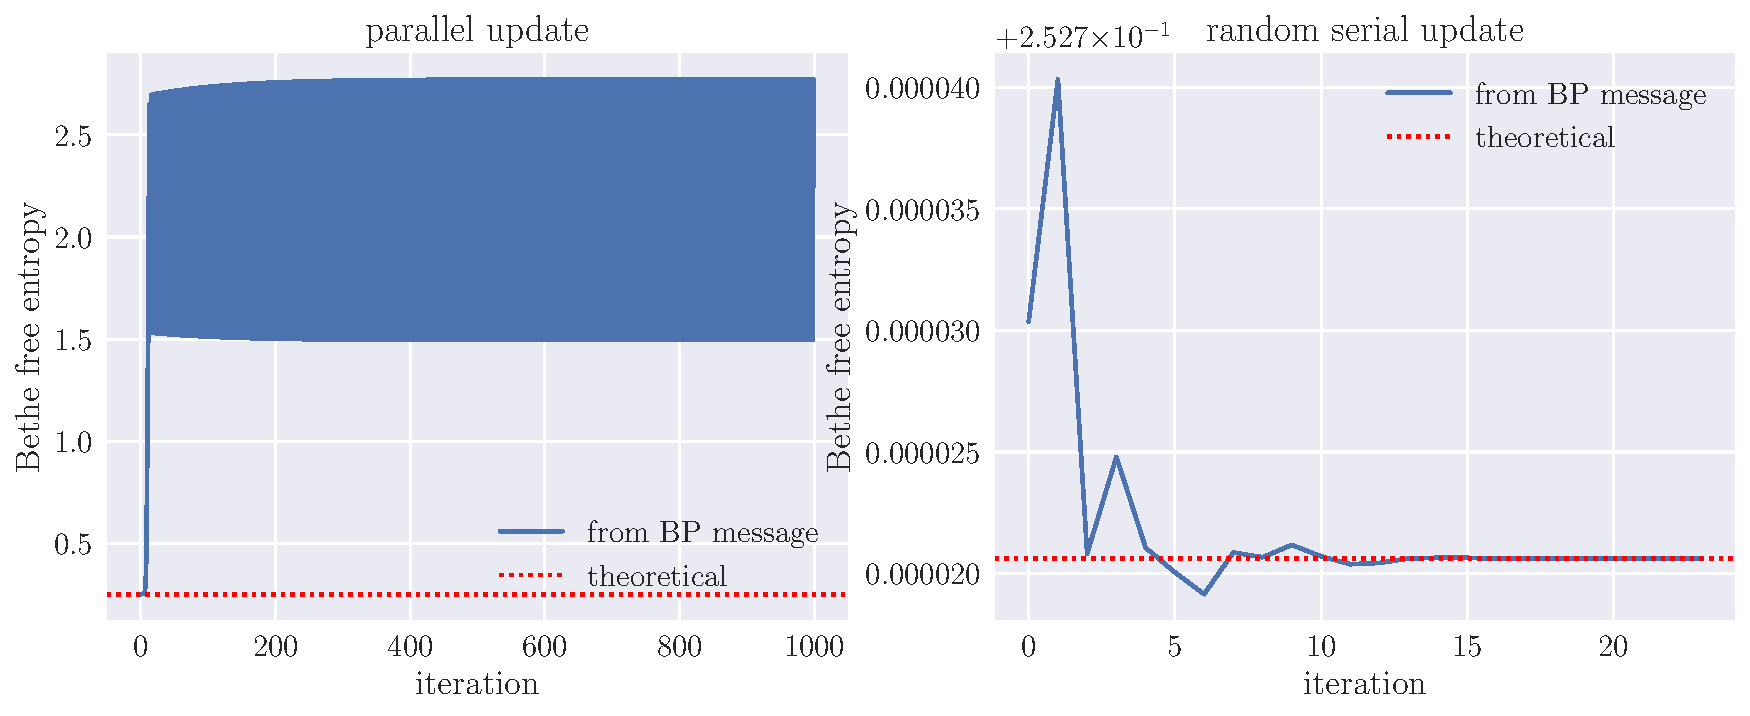
\includegraphics[width=\textwidth]{hw3/hw3_1(b)}
            \vspace{-5mm}
            \caption{Bethe free entropy trace under different BP update schedule for case $ N = 1000 $, $ \beta = 2 $, $ q = 3 $ and $ c = 5 $}
        \end{figure}
\item 
        Here I choose $ N = 200, 500, 1000, 2000 $, $ \beta = 2 $, $ q = 3 $, and $ c \in [0.1, 7] $ with step size $ 0.1 $, the BP update schedule is randomly one by one.
        For each $ c $, I drawn $ 5 $ random graphs to run BP till converge or reach $ 1000 $ iterations, and in the plot the median converge time of these five trials is plotted. 
        We can see there is a jump at $ c = 6 $.
        \begin{figure}
            \centering
            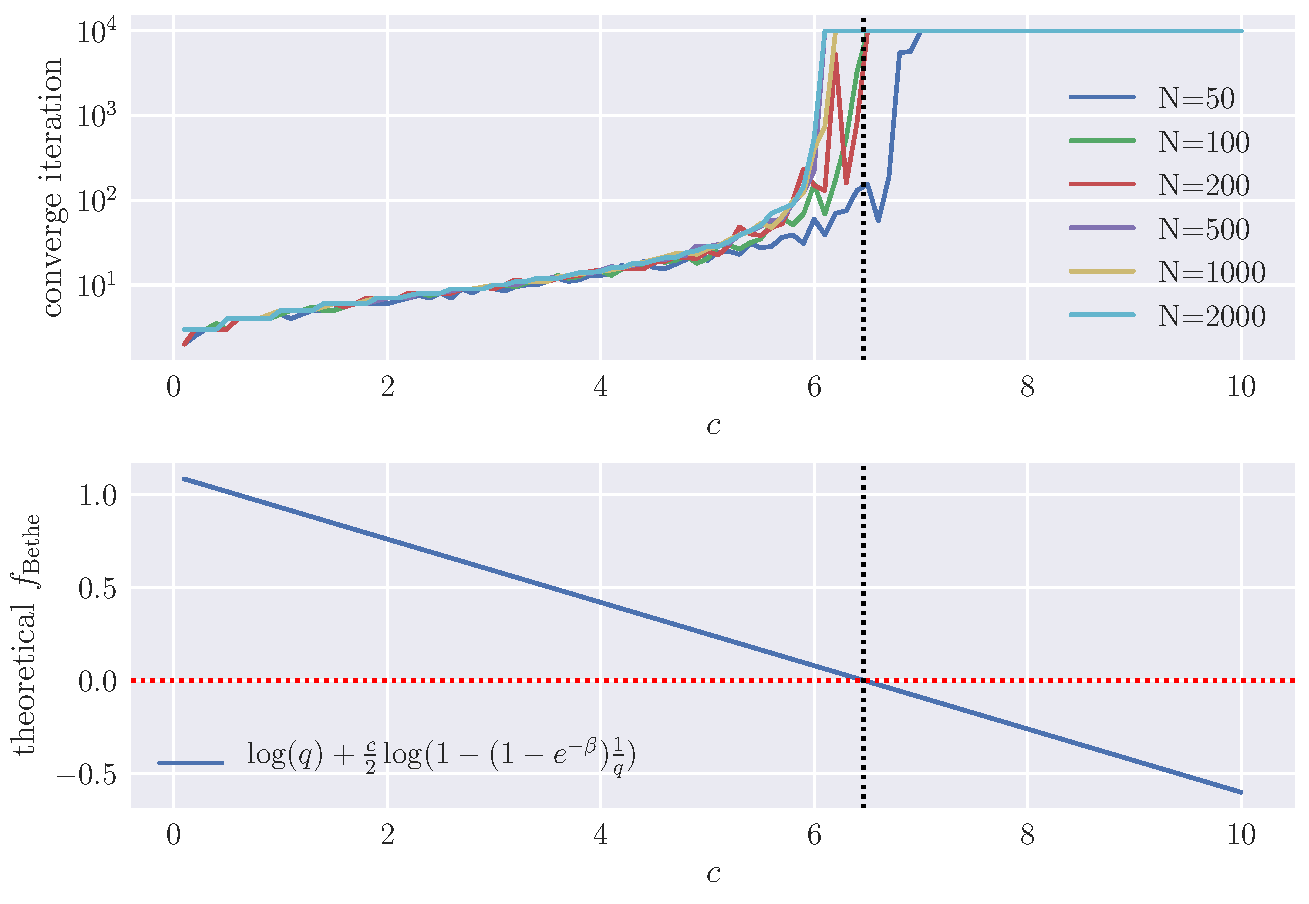
\includegraphics[width=300pt]{hw3/hw3_1(c)}
            \vspace{-5mm}
            \caption{Convergence time vs. $ c $ for the case $ N = 1000 $, $ \beta = 2 $, $ q = 3 $.}
        \end{figure}
\item   
        Here I choose $ N = 1000 $, $ \beta = 2 $, $ q = 3 $ and $ c = 5 $. And three different initializations: small perturbation from $ 1/q $, totally random, point mass on first color.
        One can see for this case they converge to same point where the Bethe free entropy is around $ 2.19 $.
        However, since BP fixed point can be viewed as the stationary point of Bethe free entropy, when Bethe free entropy has multiple stationary points, the BP evolution may converge to different fixed points, which is determined by the initialization.
        \begin{figure}
            \centering
            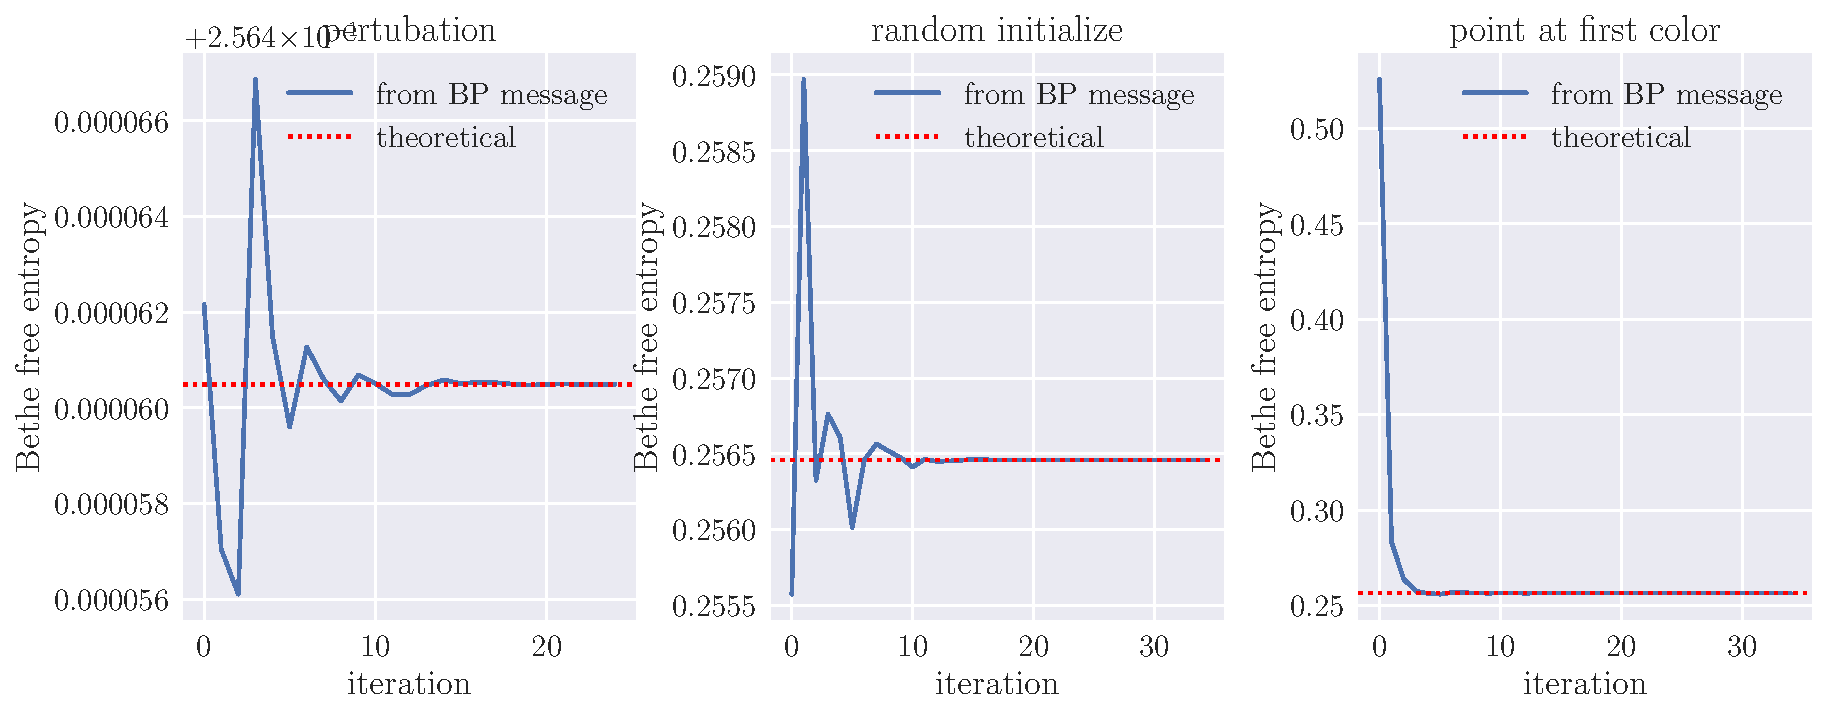
\includegraphics[width=\textwidth]{hw3/hw3_1(d)}
            \vspace{-5mm}
            \caption{Bethe free entropy trace under different initialization for various $ N $, $ \beta = 2 $, $ q = 3 $ and $ c = 5 $}
        \end{figure}
\end{enumerate}
\end{solution}


\subsection*{Concentration of the free energy in the Random Field Ising Model}

The Random Field Ising Model (RFIM) is a generalization of the Curie-Weiss model with random fields. 
Again, given $ N $ spins variables $ S_i = \pm 1 $, the Hamiltonian reads
\begin{IEEEeqnarray*}{rCl}
    \mathcal{H} \rdbrs{ \vec{S}, \vec{h} } = -N \rdbrs{ \sum_i \frac{S_i}{N} }^2 - \sum_i h_i S_i
\end{IEEEeqnarray*}
where the $ N $ values of the random fields are chosen randomly from $ \mathcal{N}(0, \Delta) $.

For a given realization of the disorder (denoting $ \vec{h} $ the ensemble of all values of $ h $), the partition function is therefore an explicit function of $ \vec{h} $:
\begin{equation*}
    F(\beta, \vec{h}) = \log \rdbrs{ Z(\beta, \vec{h}) }
\end{equation*}
\begin{enumerate}[(a)]
\item 
        Show that the function $ F(\beta,\vec{h}) $ seen as function of $ h_1 $ is a Lipschitz function with constant $ \beta $, i.e.: $ \abs{\partial_{h_1} F} \le \beta $.
\item 
        Show that the function $ F(\beta,\vec{h}) $ seen as a function of $ \vec{h} $ is Lipschitz with constant $ \beta \sqrt{N} $, i.e. that $ \abs{f(x) - f(y)} \le \beta \sqrt{N} \norm{x-y}_2 $, $ \forall\, x, y \in \mathbb{R}^n $
\item 
        Prove that the free entropy per spin (i.e. divided by $ N $) is concentrated with high probability around its mean value using the following theorem:
        Let $ (X_1,\ldots,X_n) $ be a vector of i.i.d. standard Gaussian variables, and let $ f \colon \mathbb{R}^n \to \mathbb{R} $ be $ L $-Lipschitz with respect to the Euclidean norm. 
        Then for all $ t \ge 0 $:
        \begin{equation*}
            \mathbb{P} \rdbrs{ \abs{f(X) - \mathbb{E}[f(X)]} \ge t } \le 2 \ee^{-\frac{t^2}{2L^2}}
        \end{equation*}
\end{enumerate}
\begin{solution} $\,$ 
First let's write $ F(\beta,\vec{h}) $ explicitly
\begin{IEEEeqnarray*}{rCl}
    F(\beta, \vec{h})
    &=& \log \rdbrs{ Z(\beta, \vec{h}) }
    = \log \rdbrs{ \sum_{\vec{S}} \exp \rdbrs{-\beta \mathcal{H}(\vec{S}, \vec{h})} } \\
    &=& \log \rdbrs{ \sum_{\vec{S}} \exp \rdbrs{ \beta N \rdbrs{ \sum_i \frac{S_i}{N} }^2 + \beta \sum_i h_i S_i } }
\end{IEEEeqnarray*}
\begin{enumerate}[(a)]
\item   Take partial derivative w.r.t. $ h_1 $ and note $ S_i = \pm 1 $, we have
        \begin{IEEEeqnarray*}{rCl}
            \abs{ \fracp{F(\beta, \vec{h})}{h_1} }
            &=& \abs{ \frac{ \sum_{\vec{S}}  \beta S_i \exp \rdbrs{ \beta N \rdbrs{ \sum_i \frac{S_i}{N} }^2 + \beta \sum_i h_i S_i } }{ \sum_{\vec{S}} \exp \rdbrs{ \beta N \rdbrs{ \sum_i \frac{S_i}{N} }^2 + \beta \sum_i h_i S_i } } } \\
            &\le& \beta \frac{ \sum_{\vec{S}} \abs{S_i} \exp \rdbrs{ \beta N \rdbrs{ \sum_i \frac{S_i}{N} }^2 + \beta \sum_i h_i S_i } }{ \sum_{\vec{S}} \exp \rdbrs{ \beta N \rdbrs{ \sum_i \frac{S_i}{N} }^2 + \beta \sum_i h_i S_i } }
            = \beta
        \end{IEEEeqnarray*}
\item   
        % Take gradient of $ f(\beta, \vec{h}) $ w.r.t. $ \vec{h} $, we have
        % \begin{IEEEeqnarray*}{rCl}
        %     \nabla_{\vec{h}} \, f(\beta, \vec{h})
        %     &=& \bmtx{ \fracp{f(\beta, \vec{h})}{h_1} \\ \vdots \\ \fracp{f(\beta, \vec{h})}{h_N} }
        %     = \frac{\beta}{Z(\beta,\vec{h})} 
        % \end{IEEEeqnarray*}
        Given any $ \vec{x}, \vec{y} \in \mathbb{R}^N $, we start with defining a auxiliary function $ g(t) \equiv F(\beta, t \vec{x} + (1-t) \vec{y}) $.
        Since $ F(\beta, \vec{h}) $ is a continuous function of $ \vec{h} $, by mean-value theorem, there exists $ \xi \in [0,1] $ such that
        \begin{IEEEeqnarray*}{rCl}
            F(\beta, \vec{x}) - F(\beta, \vec{y})
            &=& g(1) - g(0)
            = (1 - 0) \, g^\prime(\xi) \\
            &=& \sqbrs{ \eval{ \nabla_{\vec{h}} F(\beta, \vec{h}) }_{\vec{h} = \xi \vec{x} + (1 - \xi) \vec{y}} }^{\mathrm{T}} \eval{ \fracd{ \rdbrs{ t \vec{x} + (1-t) \vec{y} } }{t} }_{t = \xi} \\
            &=& \eval{ \bmtx{ \fracp{F(\beta, \vec{h})}{h_1} & \cdots & \fracp{F(\beta, \vec{h})}{h_N} } }_{\vec{h} = \xi \vec{x} + (1 - \xi) \vec{y}} \rdbrs{ \vec{x} - \vec{y} } \\
            &=& \sum_{i=1}^N \eval{ \fracp{F(\beta, \vec{h})}{h_i} }_{\vec{h} = \xi \vec{x} + (1 - \xi) \vec{y}} (x_i - y_i)
        \end{IEEEeqnarray*}
        Using Cauchy-Schwartz inequality and the result of part (a), we have
        \begin{IEEEeqnarray*}{rCl}
            \abs{F(\beta, \vec{x}) - F(\beta, \vec{y})}
            &=& \abs{ \sum_{i=1}^N \eval{ \fracp{F(\beta, \vec{h})}{h_i} }_{\vec{h} = \xi \vec{x} + (1 - \xi) \vec{y}} (x_i - y_i) } \\
            &\le& \sqrt{ \sum_{i=1}^N \abs{ \eval{ \fracp{F(\beta, \vec{h})}{h_i} }_{\vec{h} = \xi \vec{x} + (1 - \xi) \vec{y}} }^2 \times \sum_{i=1}^N \rdbrs{ x_i - y_i }^2 } \\
            &\le& \sqrt{ \sum_{i=1}^N \beta^2 \times \sum_{i=1}^N \rdbrs{ x_i - y_i }^2 }
            = \beta \sqrt{N} \norm{ \vec{x} - \vec{y} }_2
        \end{IEEEeqnarray*}
        Hence, we finished the proof that $ F(\beta, \vec{h}) $ is a function of $ \vec{h} $ with Lipschitz constant $ \beta \sqrt{N} $.
\item   Let $ f(\beta, \vec{h}) = F(\beta, \vec{h}) / N $ to be the free entropy per spin, From the result of part (b) we have
        \begin{equation*}
            \abs{ f(\beta, \vec{x}) - f(\beta, \vec{y}) } \le \frac{\beta}{\sqrt{N}} \norm{x-y}_2
            \quad \Rightarrow \quad
            f(\beta, \vec{h}) \text{ is } \frac{\beta}{\sqrt{N}} \text{-Lipschitz}
        \end{equation*}
        Notice that we cannot apply the theorem above directly, since our $ h_i \iid \mathcal{N}(0, \Delta) $ may not be standard Gaussian.

        For convenient, define $ \tilde{f}(\beta, \vec{\tilde{h}}) \equiv f(\beta, \sqrt{\Delta} \, \vec{\tilde{h}}) $, then we can claim by choosing $ \tilde{h}_i \iid \mathcal{N}(0, 1) $, the distribution equivalence $ \tilde{f}(\beta, \vec{\tilde{h}}) \overset{\mathrm{d}}{=} f(\beta, \vec{h}) $ holds.
        \begin{IEEEeqnarray*}{rCl}
            \abs{ \tilde{f}(\beta,\vec{x}) - \tilde{f}(\beta, \vec{y}) }
            &=& \abs{ f(\beta, \sqrt{\Delta} \, \vec{x}) - f(\beta, \sqrt{\Delta} \, \vec{y}) }
            \le \beta \sqrt{ \frac{\Delta}{N} } \norm{ \vec{x} - \vec{y} }_2 \\
            \Rightarrow& \quad & \quad
            \tilde{f}(\beta, \vec{h}) \text{ is } \beta \sqrt{ \frac{\Delta}{N} } \text{-Lipschitz}
        \end{IEEEeqnarray*}
        Now apply the above theorem: $ \rdbrs{ \tilde{h}_1, \ldots, \tilde{h}_N } $ is a vector of i.i.d. standard Gaussian variables, $ \tilde{f}(\beta, \vec{\tilde{h}}) $ is a $ \beta \sqrt{ \frac{\Delta}{N} } $-Lipschitz function of $ \vec{\tilde{h}} $ w.r.t. Euclidean norm, then
        \begin{equation*}
            \mathbb{P} \rdbrs{ \abs{ \tilde{f}(\beta, \vec{\tilde{h}}) - \mathbb{E}_{\vec{\tilde{h}}} \sqbrs{ \tilde{f}(\beta, \vec{\tilde{h}}) } } \ge t } \le 2 \ee^{-N\frac{t^2}{ 2 \beta^2 \Delta }}
        \end{equation*}
        Using the distributional equality before, we finally get
        \begin{equation*}
            \mathbb{P} \rdbrs{ \abs{ f(\beta, \vec{h}) - \mathbb{E}_{\vec{h}} \sqbrs{f(\beta, \vec{h}) } } \ge t } \le 2 \ee^{-N\frac{t^2}{ 2 \beta^2 \Delta }}
            \overset{N \to \infty}{\longrightarrow} 0
        \end{equation*}
        which means when $ N $ is large, the free entropy per spin $ f(\beta, \vec{h}) $ is concentrated around its expectation w.h.p.
\end{enumerate}
\end{solution}



\subsection*{Phase diagram}

We have seen in our lecture that the free entropy of the random field ising model is given by
\begin{equation*}
    \Phi(\beta, \Delta) 
    = \limit{N \to \infty} \frac{ \log \rdbrs{ Z(\beta, \Delta) } }{N}
    = \mathsf{Extr}_m \clbrs{ -\beta \frac{m^2}{2} + \mathbb{E}_h \sqbrs{ \log \rdbrs{ 2 \cosh(\beta(h+m)) } } }
\end{equation*}

\begin{enumerate}[(a)]
\item 
        Write the self-consistent equation that should satisfies $ m $ in order to extremize the expression
\item 
        In order to solve the self-consistent equation, you need to use a computer for computing the integral, and solving the non-linear equation. 
        Your task it plot the phase diagram as a function of $ T = 1/\beta $ and $ \Delta $
\item 
        For which value of $ T = 1/\beta $ and $ \Delta $ is $ m^* $ different than $ 0 $? 
        Does the phase transition seen in the Ising model survives in presence of a small random field?
\end{enumerate}
\begin{solution} $\,$ 
\begin{enumerate}[(a)]
\item 
        Simply take partial derivative of the expression to be extremized w.r.t. $ m $ and set it to zero
        \begin{IEEEeqnarray*}{rCl}
            0 
            &=& \fracp{}{m} \clbrs{ -\beta \frac{m^2}{2} + \mathbb{E}_h \sqbrs{ \log \rdbrs{ 2 \cosh(\beta(h+m)) } } } \\
            &=&-\beta m + \mathbb{E}_h \sqbrs{ \fracp{}{m} \log \rdbrs{ 2 \cosh(\beta(h+m)) } } \\
            &=& -\beta m + \mathbb{E}_h \sqbrs{ \beta \tanh(\beta (h+m)) }
        \end{IEEEeqnarray*}
        Hence, after arranging terms, the self-consistent equation reads
        \begin{equation*}
            m = \mathbb{E}_h \sqbrs{ \tanh(\beta(h+m)) }
        \end{equation*}
\item 
        Notice the self-consistent equation has a trivial solution $ m = 0 $, and if there is another root $ m^* $, $ -m^* $ must also be a root since the expectation is taken over $ \mathcal{N}(0, \Delta) $ which is symmetric around zero.
        Therefore, it is sufficient to search for $ m^* > 0 $.

        The phase diagram is plotted on $ T = \beta^{-1} \in [0, 2] $, $ \Delta \in [0, 1] $, where the heap map is on the value of $ m^* $.
        \begin{figure}
            \centering
            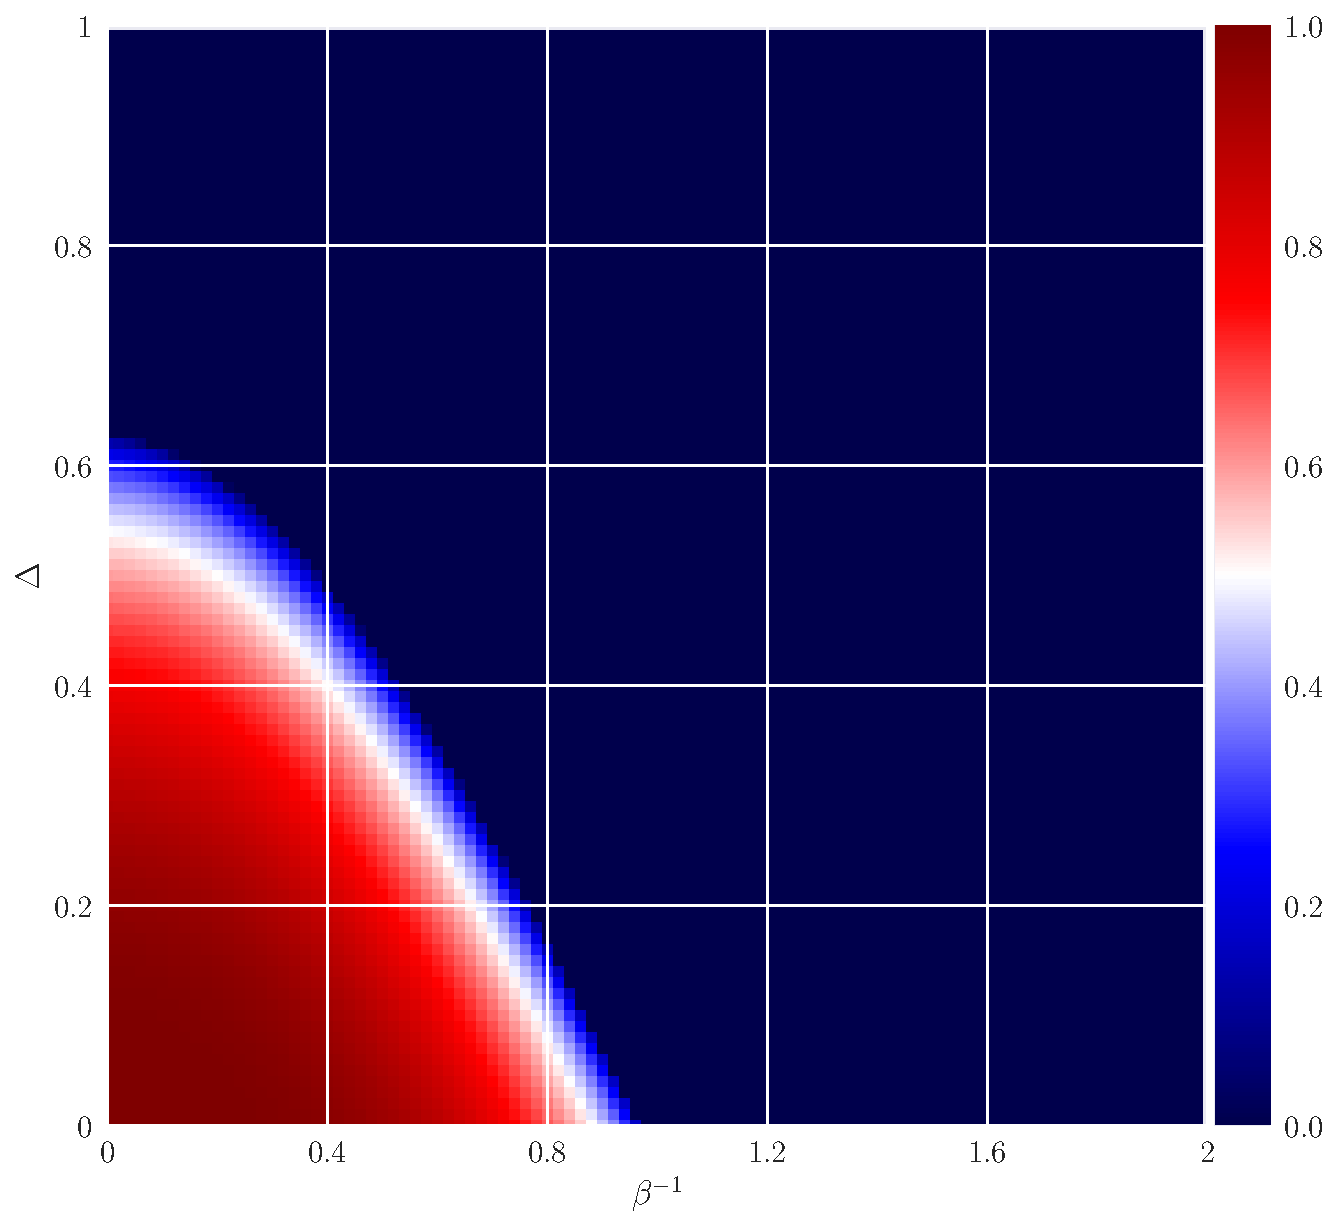
\includegraphics[width=0.49\textwidth]{hw3/hw3_2(b)}
            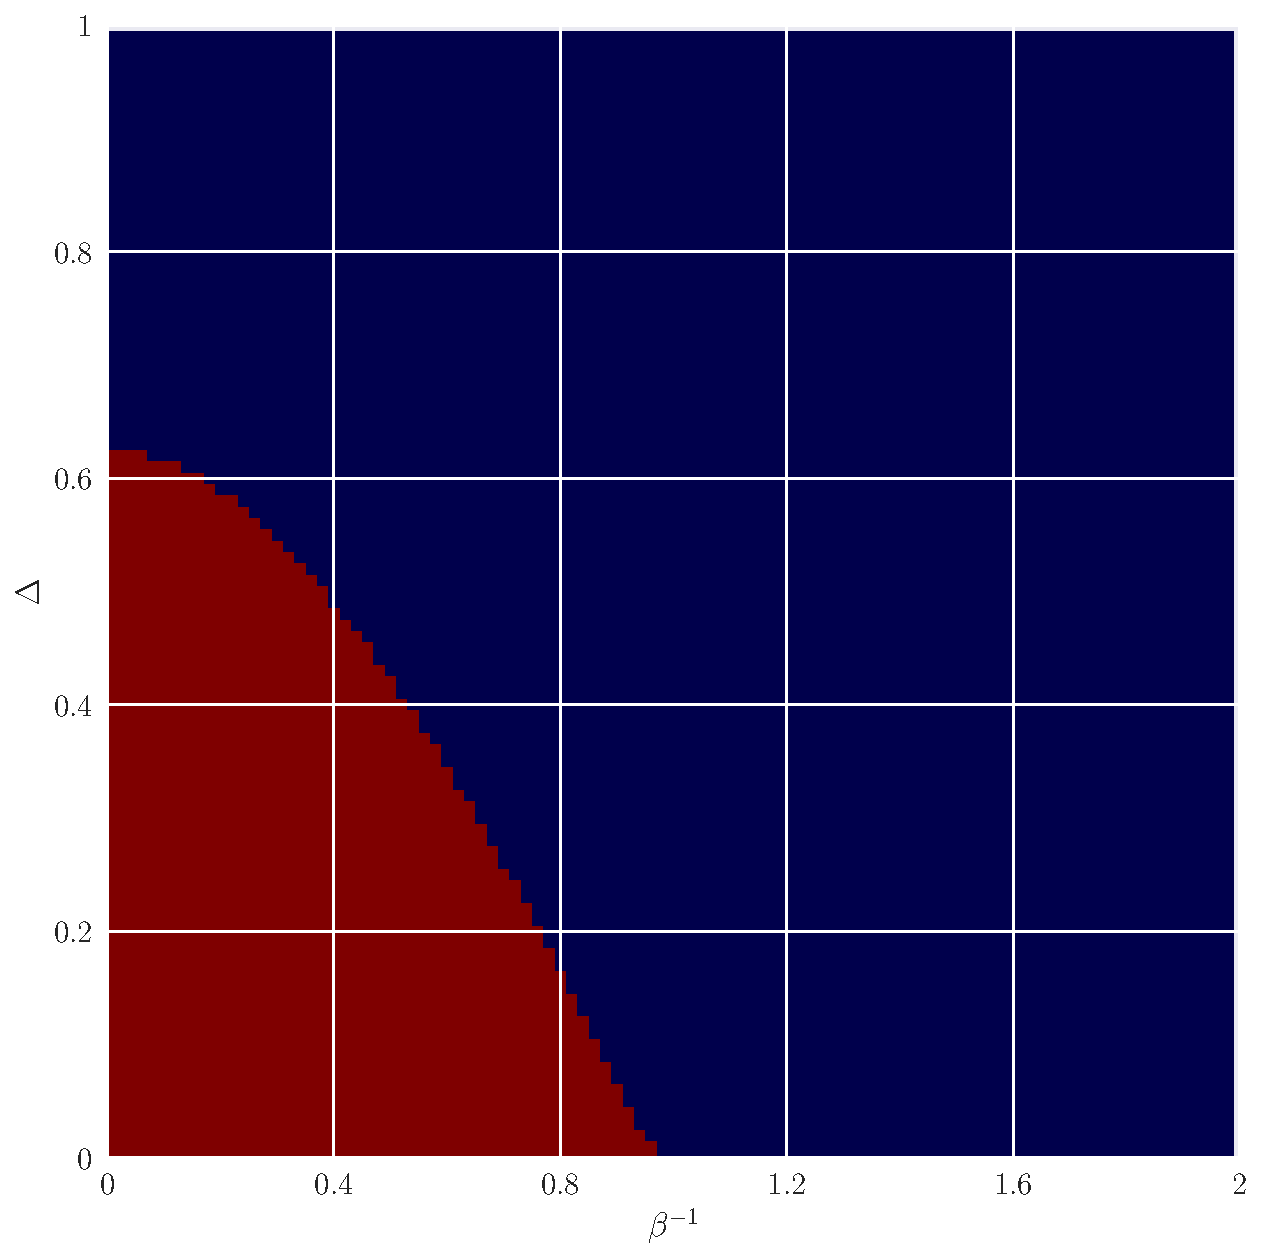
\includegraphics[width=0.45\textwidth]{hw3/hw3_2(b)2}
            \vspace{-5mm}
            \caption{Phase diagram of random field Ising model (left), binary phase digram after thresholding $ m > {10}^{-12} $ (right)}
        \end{figure}
\item   
        The exterior of left-bottom part describes the phase transition
        \begin{itemize}
        \item   When $ \Delta = 0 $, the phase transition happens at $ T = 1 $, which matches the Curie-Weiss model.
        \item   When $ T = 0 $, the phase transition happens around $ \Delta = 0.63 $.
        \end{itemize}
        Whether the phase transition survive under ``small'' random field depends on how do we define ``small'': for each $ \beta $, there exists an upper bound $ \Delta^{\mathrm{ub}}(\beta) $ such that the phase transition behavior will disappear when the variance of random field exceeds $ \Delta^{\mathrm{ub}}(\beta) $.
\end{enumerate}
\end{solution}

\subsection*{Belief-Propagation for the RFIM} 

We now consider the RFIM model on a large regular random graph with connectivity $ d $, using the Hamiltonian:
\begin{IEEEeqnarray*}{rCl}
    \mathcal{H} \rdbrs{ \clbrs{ S_i }_{i=1}^N, J, \vec{h} }
    = -\sum_{(ij) \in \mathcal{G}} J S_i S_j - \sum_i h_i S_i
\end{IEEEeqnarray*}
\begin{enumerate}[(a)]
\item
        Show that you can write the problem on a factor graph, and that the BP equations reads
        \begin{equation*}
            \chi_{S_i}^{i \to a} = \frac{\ee^{\beta h_i S_i}}{Z_\chi^{i \to a}} \prod_{b \in \partial i \setminus a} \psi_{S_i}^{b \to i}
            \quad \text{ and } \quad
            \psi_{S_i}^{b \to i} = \frac{1}{Z_\psi^{b \to i}} \sum_{ \clbrs{ S_j }_{j \in \partial b \setminus i} } \ee^{\beta J \prod_{j \in \partial b} S_j} \prod_{j \in \partial b \setminus i} \chi_{S_j}^{j \to b}
        \end{equation*}
\item   
        We shall use the following transformation:
        \begin{equation*}
            \chi_{S_i}^{i \to a} = \frac{ \ee^{\beta v^{i \to a} S_i} }{ 2 \cosh \rdbrs{ \beta h^{i \to a} } }
            \quad \text{ and } \quad
            \psi_{S_i}^{b \to i} = \frac{ \ee^{\beta u^{b \to i} S_i} }{ 2 \cosh \rdbrs{ \beta u^{b \to i} } }
        \end{equation*}
\item 
        Show that with these notations, one can rewrite BP as
        \begin{equation*}
            v^{i \to a} = h_i + \sum_{b \in \partial i \setminus a} u^{b \to i}
            \quad \text{ and } \quad
            \tanh(\beta u^{b \to i}) = \tanh(\beta J) \prod_{j \in \partial b \setminus i} \tanh \rdbrs{ \beta v^{j \to b} }
        \end{equation*}
\item 
        Finally, as in the coloring problem, show that this reduces to a set of equations on $ v^{i \to a} $ only.
        Writting the cavity magnetization as $ m^{i \to a} = \tanh \rdbrs{ \beta v^{i \to a} } $, show that in particular
        \begin{equation*}
            m^{i \to a} = \tanh \sqbrs{ \beta h_i + \atanh \rdbrs{ \sum_{b \in \partial i \setminus a} \tanh \rdbrs{ \beta J  m^{b \to i}} } }
        \end{equation*}
\item 
        Consider now the large connectivity limit $ d = N $, with $ J = 1/N $ such that the Hamiltonian reduces to the one of the fully connected model seen in the lecture and show that:
        \begin{equation*}
            m^{i \to a} = \tanh \rdbrs{ \beta h_i + \mathbb{E}_{\mathcal{G}} \sqbrs{ \beta m^{b \to i} } }
        \end{equation*}
\item 
        Show that to first order, one has $ m^{i \to a} = m^i $.
        Denoting the total magnetization as $ m = \mathbb{E}_{\mathcal{G}}[m^i] $, show that the solution of the last equation is given by the same self-consistent condition as in the lecture:
        \begin{equation*}
            m = \mathbb{E}_h \sqbrs{ \tanh(\beta h + \beta m) }
        \end{equation*}
\end{enumerate}
\begin{solution} $\,$ 
\begin{enumerate}[(a)]
\item 
        Given the Hamiltonian, we can write down the Boltzmann distribution
        \begin{equation*}
            P_{\beta, J, \vec{h}} \rdbrs{ \clbrs{ S_i }_{i=1}^N }
            = \frac{1}{Z_{J, \vec{h}}(\beta)} \ee^{ -\beta \mathcal{H} \rdbrs{ \clbrs{ S_i }_{i=1}^N, J, \vec{h} } }
            = \frac{1}{Z_{J, \vec{h}}(\beta)} \prod_i \ee^{\beta h_i S_i} \prod_{a \in \mathcal{G}} \ee^{\beta J \prod_{j \in \partial a} S_j}
        \end{equation*}
        Then, directly applying the BP update equation yields
        \begin{IEEEeqnarray*}{rCl}
            \chi_{S_i}^{i \to a}
            &=& \frac{1}{Z_\chi^{i \to a}} g_i(S_i) \prod_{b \in \partial i \setminus a} \psi_{S_i}^{b \to i}
            = \frac{ \ee^{\beta h_i S_i} }{Z_\chi^{i \to a}} \prod_{b \in \partial i \setminus a} \psi_{S_i}^{b \to i} \\
            \psi_{S_i}^{b \to i}
            &=& \frac{1}{Z_{S_i}^{b \to i}} \sum_{ \clbrs{ S_j }_{j \in \partial b \setminus i} } f_b \rdbrs{ \clbrs{ S_j }_{j \in \partial b} } \prod_{j \in \partial b \setminus i} \chi_{S_j}^{j \to b} 
            = \frac{1}{Z_{S_i}^{b \to i}} \sum_{ \clbrs{ S_j }_{j \in \partial b \setminus i} } \ee^{\beta J \prod_{j \in \partial b} S_j} \prod_{j \in \partial b \setminus i} \chi_{S_j}^{j \to b} \\
        \end{IEEEeqnarray*}
\item 
        Notice that $ S_i \in \clbrs{ \pm 1 } $,
        \begin{IEEEeqnarray*}{rCl}
            \chi_{S_i}^{i \to a}
            &=& \frac{ \ee^{\beta v^{i \to a} S_i} }{ 2 \cosh(\beta v^{i \to a}) }
            = \frac{\ee^{\beta v^{i \to a} S_i} }{ \ee^{\beta v^{i \to a} \cdot (+1)} + \ee^{\beta v^{i \to a} \cdot (-1)} }
            \quad \Rightarrow \quad
            v^{i \to a} = \frac{1}{2 \beta} \log \rdbrs{ \frac{ \chi_{+1}^{i \to a} }{ \chi_{-1}^{i \to a} } } \\
            \psi_{S_i}^{b \to i}
            &=& \frac{ \ee^{\beta u^{b \to i} S_i} }{ 2 \cosh(\beta u^{b \to i}) }
            = \frac{\ee^{\beta u^{b \to i} S_i} }{ \ee^{\beta u^{b \to i} \cdot (+1)} + \ee^{\beta u^{b \to i} \cdot (-1)} }
            \quad \Rightarrow \quad
            u^{b \to i} = \frac{1}{2 \beta} \log \rdbrs{ \frac{ \psi_{+1}^{b \to i} }{ \psi_{-1}^{b \to i} } }
        \end{IEEEeqnarray*}
        Here $ u $ and $ v $ are called \emph{log-likelihood-ratio} (LLR), which is a compact parameterization when the spin only takes two values.
\item   
        Directly apply LLR parameterization into BP equations we have
        \begin{IEEEeqnarray*}{rCl}
            v^{i \to a} 
            &=& \frac{1}{2 \beta} \log \rdbrs{ \frac{ \chi_{+1}^{i \to a} }{ \chi_{-1}^{i \to a} } } 
            = \frac{1}{2 \beta} \log \rdbrs{ \frac{ \frac{ \ee^{\beta h_i \cdot (+1)} }{Z_\chi^{i \to a}} \prod_{b \in \partial i \setminus a} \psi_{+1}^{b \to i} }{ \frac{ \ee^{\beta h_i \cdot (-1)} }{Z_\chi^{i \to a}} \prod_{b \in \partial i \setminus a} \psi_{-1}^{b \to i} } } \\
            &=& \frac{1}{2 \beta} \log \rdbrs{ \ee^{2 \beta h_i} \cdot \prod_{b \in \partial i \setminus a} \ee^{2 \beta u^{b \to i}} }
            = h_i + \prod_{b \in \partial i \setminus a} u^{b \to i} \\
            \IEEEeqnarraymulticol{3}{l}{
                \tanh \rdbrs{ \beta u^{b \to i} }
                = \frac{ \ee^{2 \beta u^{b \to i}} - 1 }{ \ee^{2 \beta u^{b \to i}} + 1 }
                = \frac{ \psi_{+1}^{b \to i} - \psi_{-1}^{b \to i} }{ \psi_{+1}^{b \to i} + \psi_{-1}^{b \to i} }
            }\nonumber\\* \quad
            &=& \frac{ \sum_{ \clbrs{ S_j }_{j \in \partial b \setminus i} } \ee^{\beta J \prod_{j \in \partial b \setminus i} S_j} \prod_{j \in \partial b \setminus i} \chi_{S_j}^{j \to b} - \sum_{ \clbrs{ S_j }_{j \in \partial b \setminus i} } \ee^{-\beta J \prod_{j \in \partial b \setminus i} S_j} \prod_{j \in \partial b \setminus i} \chi_{S_j}^{j \to b} }{ \sum_{ \clbrs{ S_j }_{j \in \partial b \setminus i} } \ee^{\beta J \prod_{j \in \partial b \setminus i} S_j} \prod_{j \in \partial b \setminus i} \chi_{S_j}^{j \to b} + \sum_{ \clbrs{ S_j }_{j \in \partial b \setminus i} } \ee^{-\beta J \prod_{j \in \partial b \setminus i} S_j} \prod_{j \in \partial b \setminus i} \chi_{S_j}^{j \to b} } \\
            &=& \frac{ \sum_{ \clbrs{ S_j }_{j \in \partial b \setminus i} } \rdbrs{ \ee^{\beta J \prod_{j \in \partial b \setminus i} S_j} - \ee^{-\beta J \prod_{j \in \partial b \setminus i} S_j} } \prod_{j \in \partial b \setminus i} \ee^{2 \beta v^{j \to b} \delta_{S_j, +1}} }{ \sum_{ \clbrs{ S_j }_{j \in \partial b \setminus i} } \rdbrs{ \ee^{\beta J \prod_{j \in \partial b \setminus i} S_j} + \ee^{-\beta J \prod_{j \in \partial b \setminus i} S_j} } \prod_{j \in \partial b \setminus i} \ee^{2 \beta v^{j \to b} \delta_{S_j, +1}} } \\
            &=& \frac{ \rdbrs{ \ee^{\beta J} - \ee^{-\beta J} } \sqbrs{ \sum_{ \clbrs{ S_j }_{j \in \partial b \setminus i} }^{\mathrm{even}} \ee^{2 \beta \sum_{j \in \partial b \setminus i} v^{j \to b} \delta_{S_j, +1}} - \sum_{ \clbrs{ S_j }_{j \in \partial b \setminus i} }^{\mathrm{odd}} \ee^{2 \beta \sum_{j \in \partial b \setminus i} v^{j \to b} \delta_{S_j, +1}} } }{ \rdbrs{ \ee^{\beta J} + \ee^{-\beta J} } \sqbrs{ \sum_{ \clbrs{ S_j }_{j \in \partial b \setminus i} }^{\mathrm{even}} \ee^{2 \beta \sum_{j \in \partial b \setminus i} v^{j \to b} \delta_{S_j, +1}} + \sum_{ \clbrs{ S_j }_{j \in \partial b \setminus i} }^{\mathrm{odd}} \ee^{2 \beta \sum_{j \in \partial b \setminus i} v^{j \to b} \delta_{S_j, +1}} } } \\
            &=& \tanh(\beta J) \cdot \frac{ \frac{ \prod_{j \in \partial b \setminus i} \rdbrs{ \ee^{2 \beta v^{j \to b}} + 1} + \prod_{j \in \partial b \setminus i} \rdbrs{ \ee^{2 \beta v^{j \to b}} - 1} }{2} - \frac{ \prod_{j \in \partial b \setminus i} \rdbrs{ \ee^{2 \beta v^{j \to b}} + 1} - \prod_{j \in \partial b \setminus i} \rdbrs{ \ee^{2 \beta v^{j \to b}} - 1} }{2} }{ \frac{ \prod_{j \in \partial b \setminus i} \rdbrs{ \ee^{2 \beta v^{j \to b}} + 1} + \prod_{j \in \partial b \setminus i} \rdbrs{ \ee^{2 \beta v^{j \to b}} - 1} }{2} + \frac{ \prod_{j \in \partial b \setminus i} \rdbrs{ \ee^{2 \beta v^{j \to b}} + 1} - \prod_{j \in \partial b \setminus i} \rdbrs{ \ee^{2 \beta v^{j \to b}} - 1} }{2} } \\
            &=& \tanh(\beta J) \cdot \frac{ \prod_{j \in \partial b \setminus i} \rdbrs{ \ee^{2 \beta v^{j \to b}} - 1 } }{ \prod_{j \in \partial b \setminus i} \rdbrs{ \ee^{2 \beta v^{j \to b}} + 1 } }
            = \tanh(\beta J) \cdot \prod_{j \in \partial b \setminus i} \tanh \rdbrs{ \beta v^{j \to b} }
        \end{IEEEeqnarray*}
        where $ \sum_{ \clbrs{ S_j }_{j \in \partial b \setminus i} }^{\mathrm{even}}, \sum_{ \clbrs{ S_j }_{j \in \partial b \setminus i} }^{\mathrm{odd}} $ are summed over $ \clbrs{ S_j }_{j \in \partial b \setminus i} $ but restricted to terms with $ \prod_{j \in \partial b \setminus i} S_i = +1 $ and $ -1 $, respectively.
\item 
        Since in this model, all interactions are pairwise, the BP equations can be simplified as
        \begin{IEEEeqnarray*}{rCl}
            v^{i \to (ij)} = h_i + \sum_{k \in \partial^* i \setminus j} u^{(ik) \to i}, \quad
            \tanh(\beta u^{(ij) \to j}) = \tanh(\beta J) \tanh \rdbrs{ \beta v^{i \to (ij)} }, \quad \forall\, (ij) \in \mathcal{G}
        \end{IEEEeqnarray*}
        By letting $ m^{i \to (ij)} = \tanh \rdbrs{ \beta v^{i \to (ij)} } $ we have
        \begin{IEEEeqnarray*}{rCl}
            m^{i \to (ij)}
            &=& \tanh \rdbrs{ \beta v^{i \to (ij)} }
            = \tanh \rdbrs{ \beta h_i + \beta \sum_{k \in \partial^* i \setminus j} u^{(ik) \to i} } \\
            &=& \tanh \rdbrs{ \beta h_i + \sum_{k \in \partial^* i \setminus j} \atanh \rdbrs{ \tanh(\beta J) \tanh \rdbrs{ \beta v^{k \to (ik)} } } } \\
            &=& \tanh \rdbrs{ \beta h_i + \sum_{k \in \partial^* i \setminus j} \atanh \rdbrs{ \tanh(\beta J) m^{k \to (ik)} } }
        \end{IEEEeqnarray*}
\item 
        In the large connectivity limit $ d = N $, the graph grows to fully connected. 
        Besides, as $ J = 1/N $, the Hamiltonian reduces to the RFIM in the lecture
        \begin{equation*}
            \mathcal{H} \rdbrs{ \clbrs{ S_i }_{i=1}^N, \vec{h} }
            = -\frac{1}{N} \sum_{i,j} S_i S_j - \sum_i h_i S_i
        \end{equation*}
        Notice that when $ x \to 0 $, $ \tanh(x) = x + \mathrm{O}(x^3) $, $ \atanh(x) = x + \mathrm{O}(x^3) $.
        Therefore, in the large-$ N $ limit, the cavity magnetization equation for the whole random graph ensemble becomes
        \begin{IEEEeqnarray*}{rCl}
            m^{i \to (ij)}
            &=& \tanh \rdbrs{ \beta h_i + \mathbb{E}_{\mathcal{G}} \sqbrs{ \sum_{k \in \partial^* i \setminus j} \atanh \rdbrs{ \tanh(\beta J) m^{k \to (ik)} } } } \\
            &=& \tanh \rdbrs{ \beta h_i + \mathbb{E}_{\mathcal{G}} \sqbrs{ \sum_{ \substack{k=1 \\ k \notin \clbrs{ i, j }} }^N \atanh \rdbrs{ \tanh \rdbrs{ \frac{\beta}{N} } m^{k \to (ik)} } } } \\
            &=& \tanh \rdbrs{ \beta h_i + \mathbb{E}_{\mathcal{G}} \sqbrs{ \sum_{ \substack{k=1 \\ k \notin \clbrs{ i, j }} }^N \atanh \rdbrs{ \frac{\beta}{N} m^{k \to (ik)} } } } \\
            &=& \tanh \rdbrs{ \beta h_i + \mathbb{E}_{\mathcal{G}} \sqbrs{ \sum_{ \substack{k=1 \\ k \notin \clbrs{ i, j }} }^N \frac{\beta}{N} m^{k \to (ik)} } } \\
            &=& \tanh \rdbrs{ \beta h_i + \mathbb{E}_{\mathcal{G}} \sqbrs{\beta m^{k \to (ik)} } }
        \end{IEEEeqnarray*}
\item   
        Compare equations between $ m^i $ and $ m^{i \to (ij)} $, and apply Taylor expansion around $ m^{i \to (ij)} $ we have
        \begin{IEEEeqnarray*}{rCl}
            m^i
            &=& \tanh \rdbrs{ \beta h_i + \mathbb{E}_{\mathcal{G}} \sqbrs{ \sum_{ \substack{k=1 \\ k \ne i} }^N \frac{\beta}{N} m^{k \to (ik)} } } \\
            &=& \tanh \rdbrs{ \atanh \rdbrs{ m^{i \to (ij)} } + \frac{\beta}{N} \mathbb{E}_{\mathcal{G}} \sqbrs{ m^{j \to (ij)} } } \\
            &=& m^{i \to (ij)} + \frac{\beta}{N} \rdbrs{ 1 - \sqbrs{ m^{i \to (ij)} }^2 } \mathbb{E}_{\mathcal{G}} \sqbrs{ m^{j \to (ij)} } + \mathrm{O}(N^{-2})
        \end{IEEEeqnarray*}
        which indicates that to the first order $ m^{i \to (ij)} = m^i $.
        Use this conclusion and result of part (e), we can claim that to the first order
        \begin{equation*}
            m^i = \tanh \rdbrs{ \beta h_i + \beta \mathbb{E}_{\mathcal{G}}[m^k] }
        \end{equation*}
        Note $ m = \mathbb{E}_{\mathcal{G}}[m^i] $ does not depend on $ \mathcal{G} $, taking expectation over $ \mathcal{G} $ and $ \vec{h} $ on both sides yields
        \begin{IEEEeqnarray*}{rCl}
            m
            &=& \mathbb{E}_{\vec{h}} \sqbrs{ \frac{1}{N} \sum_i m }
            = \frac{1}{N} \mathbb{E}_{\vec{h}} \sqbrs{ \sum_i \mathbb{E}_{\mathcal{G}}[m^i] }
            = \frac{1}{N} \mathbb{E}_{\mathcal{G}} \sqbrs{ \sum_i \mathbb{E}_{h_i}[m^i] } \\
            &=& \frac{1}{N} \mathbb{E}_{\mathcal{G}} \sqbrs{ \sum_i \mathbb{E}_{h_i} \sqbrs{ \tanh \rdbrs{ \beta h_i + \beta \mathbb{E}_{\mathcal{G}}[m^k] } } } \\
            &=& \frac{1}{N} \mathbb{E}_{\mathcal{G}} \sqbrs{ \sum_i \mathbb{E}_{h_i} \sqbrs{ \tanh \rdbrs{ \beta h_i + \beta m } } }
            = \mathbb{E}_h \sqbrs{ \tanh \rdbrs{ \beta (h+m) } }
        \end{IEEEeqnarray*}
        which is same as the self-consistent condition in the lecture and finishes the proof.
\end{enumerate}
\end{solution}
\end{document}